\documentclass[12pt]{article}
\usepackage[english]{babel}
\usepackage{natbib}
\usepackage{url}
\usepackage[utf8x]{inputenc}
\usepackage{amsmath}
\usepackage{graphicx}
\graphicspath{{images/}}
\usepackage{parskip}
\usepackage{fancyhdr}
\usepackage{vmargin}
\usepackage{float}
\usepackage{graphicx}
\usepackage{breqn}
\usepackage{rotating}


\setmarginsrb{3 cm}{2.5 cm}{3 cm}{2.5 cm}{1 cm}{1.5 cm}{1 cm}{1.5 cm}

\title{TP 2}								% Title
\author{Zins Pierre 1863527}						% Author
\date{Février 20, 2017}							% Date

\makeatletter
\let\thetitle\@title
\let\theauthor\@author
\let\thedate\@date
\makeatother

\pagestyle{fancy}
\fancyhf{}
%\rhead{\theauthor}
\lhead{\thetitle}
\cfoot{\thepage}

\begin{document}

%%%%%%%%%%%%%%%%%%%%%%%%%%%%%%%%%%%%%%%%%%%%%%%%%%%%%%%%%%%%%%%%%%%%%%%%%%%%%%%%%%%%%%%%%

\begin{titlepage}
	\centering
    \vspace*{0.5 cm}
    \includegraphics[scale = 0.9]{poly_logo.png}\\[1.0 cm]	% University Logo
    \textsc{\LARGE Polytechnique Montréal}\\[2.0 cm]	% University Name
	\textsc{\Large INF8225 }\\[0.5 cm]				% Course Code
	\textsc{Intelligence artificielle : modèles probabilistes et apprentissage}\\[0.5 cm]				% Course Name
	\rule{\linewidth}{0.2 mm} \\[0.4 cm]
	{ \huge \bfseries \thetitle}\\
	\rule{\linewidth}{0.2 mm} \\[1.5 cm]
	
	\begin{minipage}{0.4\textwidth}
		\begin{flushleft} \large
			\emph{Auteur:}\\
			\theauthor
			\end{flushleft}
			\end{minipage}~
			\begin{minipage}{0.4\textwidth}
			\begin{flushright} \large
												% Your Student Number
		\end{flushright}
	\end{minipage}\\[2 cm]
	
	{\large \thedate}\\[2 cm]
 
	\vfill
	
\end{titlepage}

%%%%%%%%%%%%%%%%%%%%%%%%%%%%%%%%%%%%%%%%%%%%%%%%%%%%%%%%%%%%%%%%%%%%%%%%%%%%%%%%%%%%%%%%%

%%%%%%%%%%%%%%%%%%%%%%%%%%%%%%%%%%%%%%%%%%%%%%%%%%%%%%%%%%%%%%%%%%%%%%%%%%%%%%%%%%%%%%%%%

%\section{Appendices}
Au travers de ce TP, j'ai pu me familiariser avec l'apprentissage automatique au travers de la méthode de régression logistique. Pour cette dernière, j'ai utilisé deux méthodes d'optimisation : par "batch" et par "mini-batch". J'ai programmé cela en Python avec \textit{Scipy} et \textit{Numpy}.
Mon implémentation est décrite en détails aux travers des commentaires dans mon code.

Pour les différentes étapes, j'ai suivi les éléments fournis dans le sujet. \\
La descente de gradient (ba	tch ou mini-batch) s'arrête lorsque la différence entre la précision sur l'ensemble de validation de deux itérations successives est inférieure à un certain seuil (j'ai fixé ce seuil à 0.001).

\section{Batch}
Pour cette version de la descente de gradient, les paramètres sont mis à jour après le calcul du gradient sur l'ensemble d'apprentissage à chaque itération.
A chaque itération, je la calcule sur l'ensemble d'apprentissage et de validation. Une fois que la descente de gradient a convergé, je calcule la précision finale sur l'ensemble de test.

J'ai pu afficher sur le même graphe, l'évolution des précisions pendant le processus d'optimisation. J'ai également pu faire varier le taux d'apprentissage afin de voir l'impact de ce dernier.
J'ai affiché les graphes pour trois taux d'apprentissage : 
\begin{itemize}
\item 0.0005 : taux normal de base
\item 0.001 : pour mesurer l'impact d'un taux plus grand
\item 0.0001 : pour mesurer l'impact d'un taux plus faible
\end{itemize}
Pour chacun d'entre eux, j'ai affiché un graphe avec la précision pour l'ensemble de validation, de test et d'apprentissage et un second graphe présentant la log vraisemblance. 

\begin{figure}[H]
\begin{center}
	\includegraphics[scale=0.8]{img/b_0_0005.png}
	\caption{Précision batch : taux = 0.0005}
\end{center}
\end{figure}
\begin{figure}[H]
\begin{center}
	\includegraphics[scale=0.8]{img/b_0_001.png}
	\caption{Précision batch : taux = 0.001}
\end{center}
\end{figure}
\begin{figure}[H]
\begin{center}
	\includegraphics[scale=0.8]{img/b_0_0001.png}
	\caption{Précision batch : taux = 0.0001}
\end{center}
\end{figure}
Voici maintenant les graphes de la log vraisemblance en fonction du taux d'apprentissage.
\begin{figure}[H]
\begin{center}
	\includegraphics[scale=0.8]{img/b_0_0005_logv.png}
	\caption{Log-vraisemblance batch : taux = 0.0005}
\end{center}
\end{figure}
\begin{figure}[H]
\begin{center}
	\includegraphics[scale=0.8]{img/b_0_001_logv.png}
	\caption{Log-vraisemblance  batch : taux = 0.001}
\end{center}
\end{figure}
\begin{figure}[H]
\begin{center}
	\includegraphics[scale=0.8]{img/b_0_0001_logv.png}
	\caption{Log-vraisemblance  batch : taux = 0.0001}
\end{center}
\end{figure}

On remarque que le taux d'apprentissage a un impact important sur la vitesse de l'apprentissage. L'apprentissage va plus vite quand le taux est plus élevé.
\begin{itemize}
\item taux = 0.001 $\Rightarrow$ convergence au bout de 8-10 itérations
\item taux = 0.0005 $\Rightarrow$ convergence au bout de 10-12 itération
\item taux = 0.0001 $\Rightarrow$ convergence au bout de 25-30 itérations
\end{itemize}
On a donc plutôt intérêt à choisir un taux d'apprentissage relativement élevé. Cependant, cela impacte le bon fonctionnement de la descente de gradient. Un taux trop élevé peut entraîner une divergence, et la précision va décroître sans jamais converger. On peut d'ailleurs remarquer une "réduction" de la précision vers la $4^{eme}$ itération avec le taux le plus grand (0.001). 
\\ \linebreak
Par ailleurs, les graphes ont été réalisés avec des paramètres \textit{Theta} et des ensembles de test, validation et apprentissage initialisés différemment. Il est donc compréhensible d'avoir des valeurs finales de précision ou de log-vraisemblance différentes. Théoriquement, avec la même initialisation, un taux d'apprentissage plus faible devrait permettre de mieux minimiser la fonction de perte, et donc offrir une meilleure précision.
\\
Concernant l'arrêt de la descente de gradient, j'ai conservé un seuil à 0.001. A partir de là, on peut supposer que la valeur de la précision n'évoluera plus de manière significative.
\\ \linebreak
Au niveaux des résultats pour les différents ensembles, on remarque que cela est variable. Il n'y a pas d'ensemble pour lequel la précision finale est toujours meilleure que les autres. Les trois valeurs sont toujours proches, aux alentours de 80\%. Normalement, on pourrait s'attendre à une meilleure précision sur les ensembles d'apprentissage et de validation que sur celui de test. Cependant, j'ai ajouté un terme de régularisation qui va permettre d'empêcher le sur-apprentissage. Ainsi, il peut être normal d'obtenir un résultat meilleur sur l'ensemble de test, par rapport aux deux autres.
\\ \linebreak
Finalement, j'ai aussi ajouté le \textit{momentum} pour la descente de gradient, ce qui doit permettre d'avoir une convergence plus fluide en empêchant les oscillations. Cela va donc aussi permettre une convergence plus rapide.
Il est facile de voir l'impact de ce dernier. J'ai réalisé les mesures avec les mêmes paramètres et les même valeurs initiales pour Theta. \\ Avec un taux d'apprentissage relativement grand (0.001), la descente de gradient a tendance à présenter des petites oscillations (régressions).

\begin{figure}[H]
\begin{center}
	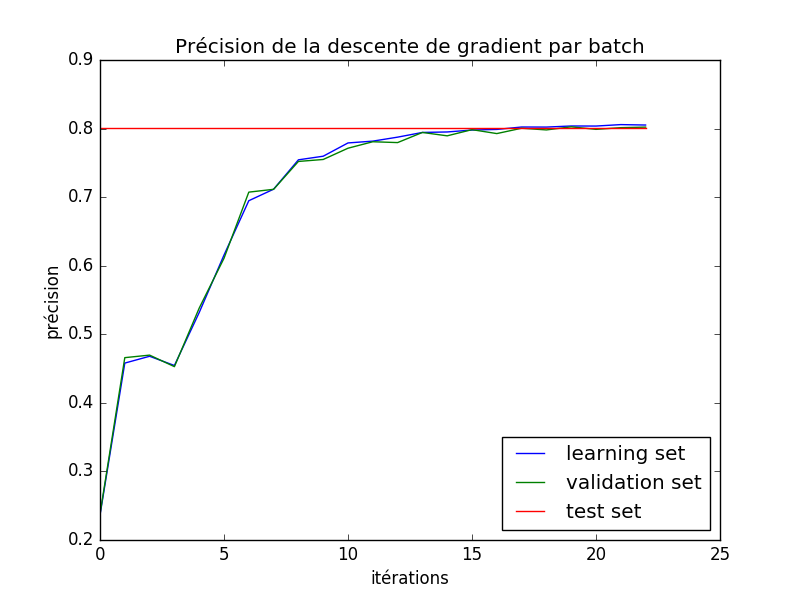
\includegraphics[scale=0.8]{img/momentum_off.png}
	\caption{Précision sans momentum}
\end{center}
\end{figure}

En ajoutant le momentum, ces oscillations vont disparaîtres. La précision finale obtenue est exactement la même, mais avec un \textit{momentum} la précision va évoluer de manière fluide sans régression. On a par conséquent un gain de temps : convergence aux alentours de 15-20 itérations sans \textit{momentum} contre 10 avec \textit{momentum}.
\begin{figure}[H]
\begin{center}
	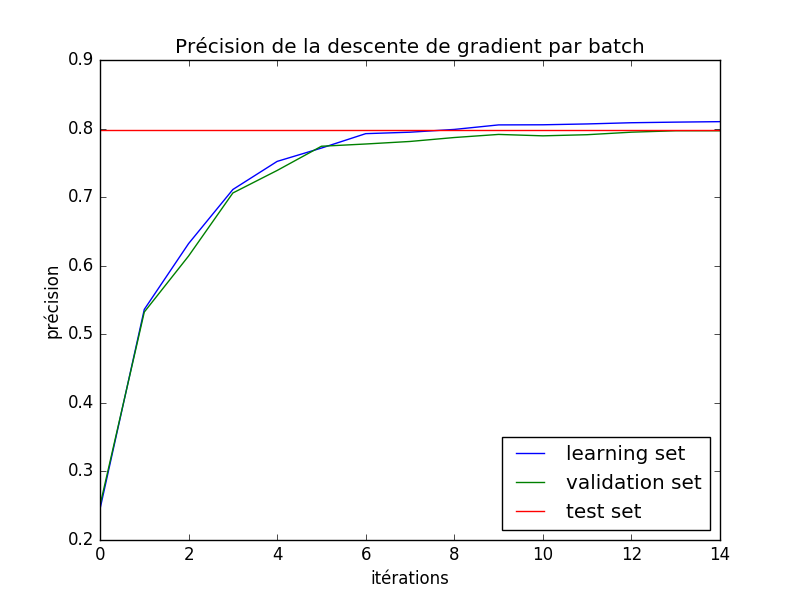
\includegraphics[scale=0.8]{img/momentum_on.png}
	\caption{Précision avec momentum}
\end{center}
\end{figure}


\section{Mini-batch}
Pour la version par mini-batch, l'ensemble d'apprentissage est découpé en plusieurs "mini-batchs" différents (20 dans ce TP). Dans ce cas, la mise à jour des paramètres Theta se fait plus régulièrement, à chaque traitement d'un mini-batch. 

J'ai pu calculer la précision sur les ensembles d'apprentissage et de validation durant la descente de gradient et la précision sur l'ensemble de test une fois le processus terminé. J'ai pu différencier, une mesure à chaque itération pour chaque mini-batch (boucle intérieure sur les mini-batch) et une mesure à chaque époque (boucle extérieure). Le premier cas propose une meilleure précision, puisque nous réalisons beaucoup plus de mesures, mais globalement il s'agit des même résultats.
J'ai également mesuré la vraisemblance, à chaque époque.\\

Concernant le taux d'apprentissage, je n'ai pas pris une valeur constante comme dans le cas précédent. Pour la version par mini-batch, il est conseillé d'avoir un taux d'apprentissage qui dépend du "temps" (des itérations dans le processus d'optimisation). Il est avantageux d'avoir un taux relativement grand au départ et plus petit par la suite. Voici le taux que j'ai choisi : 
\[\frac{C1}{t+C2}\]
De cette manière, le taux aura une valeur initiale puis va progressivement diminuer. J'ai fait des mesures pour deux taux différents. Pour le premier cas, j'ai $C1 = 1 et C2 = 1$ et pour le second $C1 = 5 et C2 = 1$. Ainsi le second taux est aura une valeur supérieure au premier pour tout t.
Pour les deux cas, j'affiche la précision mesurée à chaque époque, la précision mesurée à chaque mini-batch et la log-vraisemblance.

\begin{figure}[H]
\begin{center}
	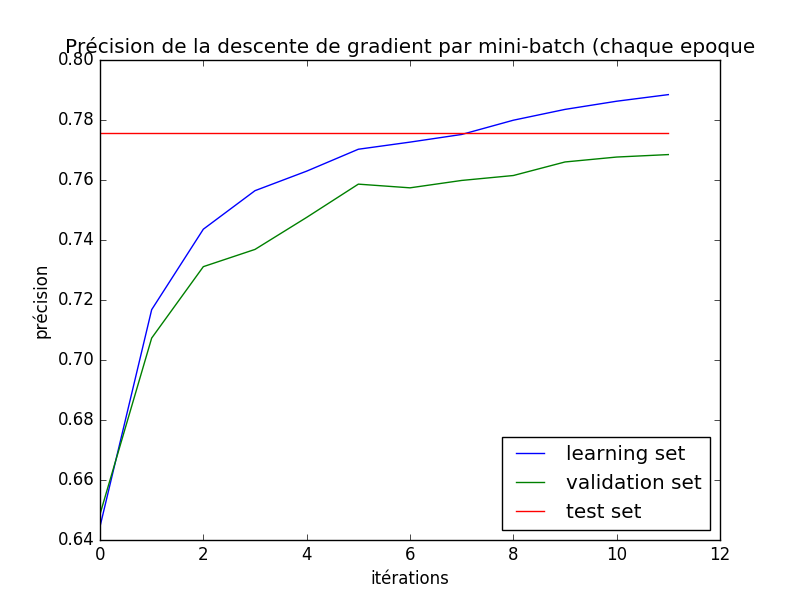
\includegraphics[scale=0.8]{img/mb_1_1.png}
	\caption{Précision mini-batch (chaque époque), taux = $\frac{1}{t+1}$}
\end{center}
\end{figure}
\begin{figure}[H]
\begin{center}
	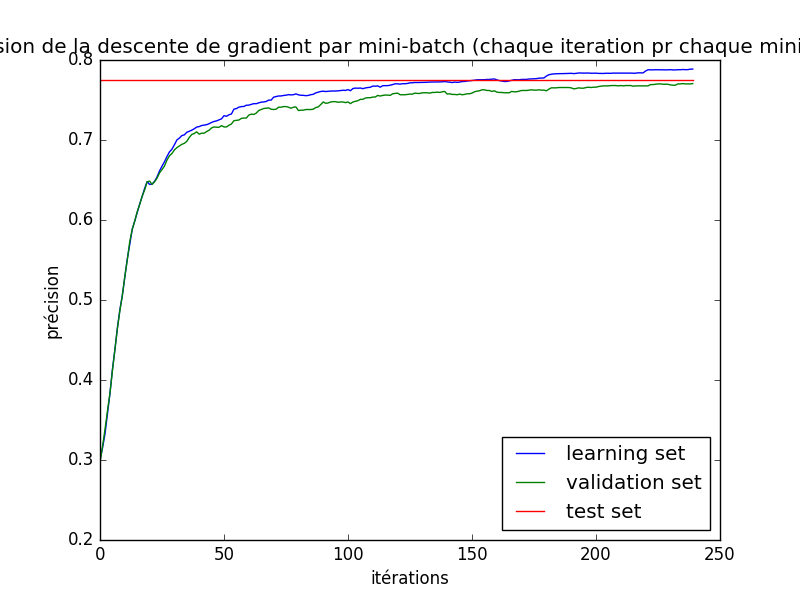
\includegraphics[scale=0.8]{img/mb_1_1_iteration_mb.png}
	\caption{Précision mini-batch (chaque mini-batch), taux = $\frac{1}{t+1}$}
\end{center}
\end{figure}
\begin{figure}[H]
\begin{center}
	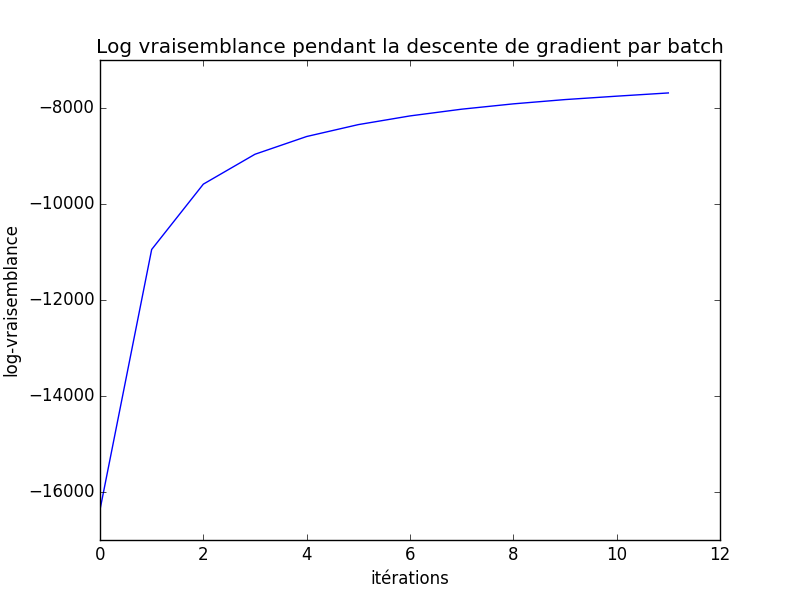
\includegraphics[scale=0.8]{img/mb_1_1_logv.png}
	\caption{Log-vraisemblance, taux = $\frac{1}{t+1}$}
\end{center}
\end{figure}
\begin{figure}[H]
\begin{center}
	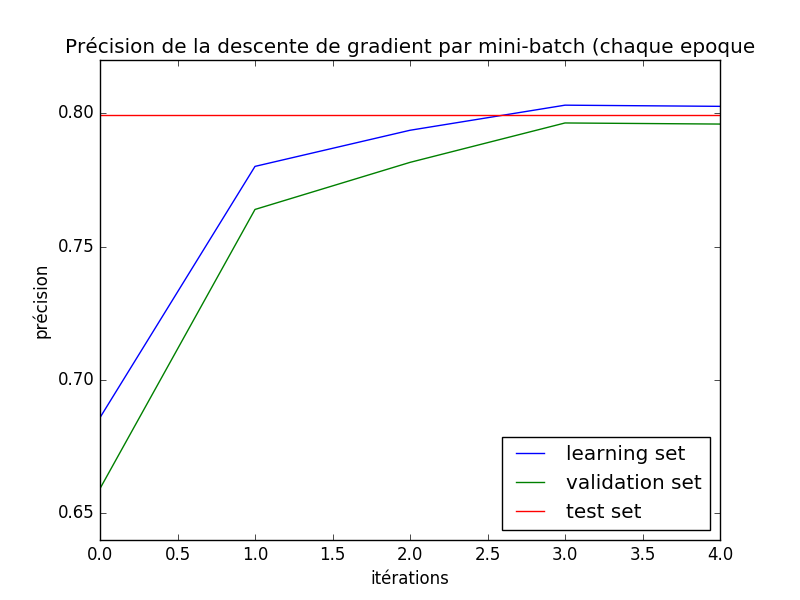
\includegraphics[scale=0.8]{img/mb_5_1.png}
	\caption{Précision mini-batch (chaque époque), taux = $\frac{5}{t+1}$}
\end{center}
\end{figure}
\begin{figure}[H]
\begin{center}
	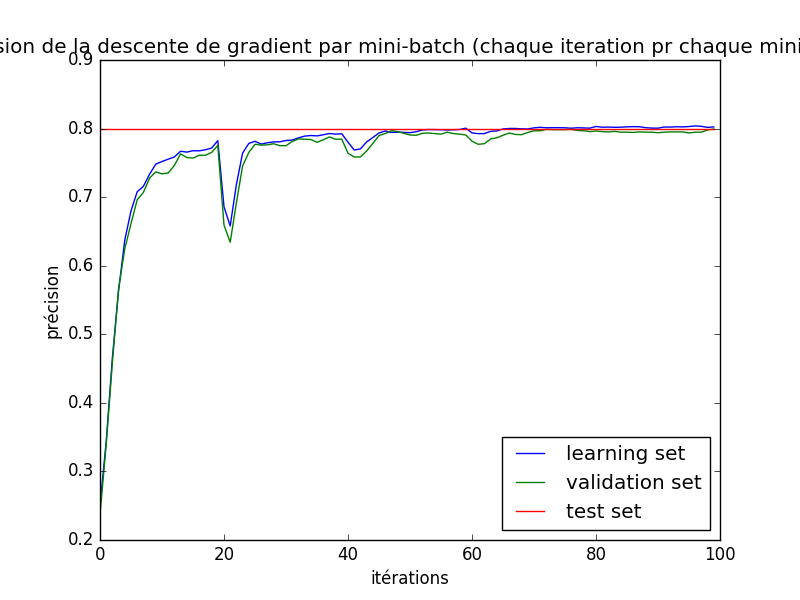
\includegraphics[scale=0.8]{img/mb_5_1_iteration_mb.png}
	\caption{Précision mini-batch (chaque mini-batch), taux = $\frac{5}{t+1}$}
\end{center}
\end{figure}
\begin{figure}[H]
\begin{center}
	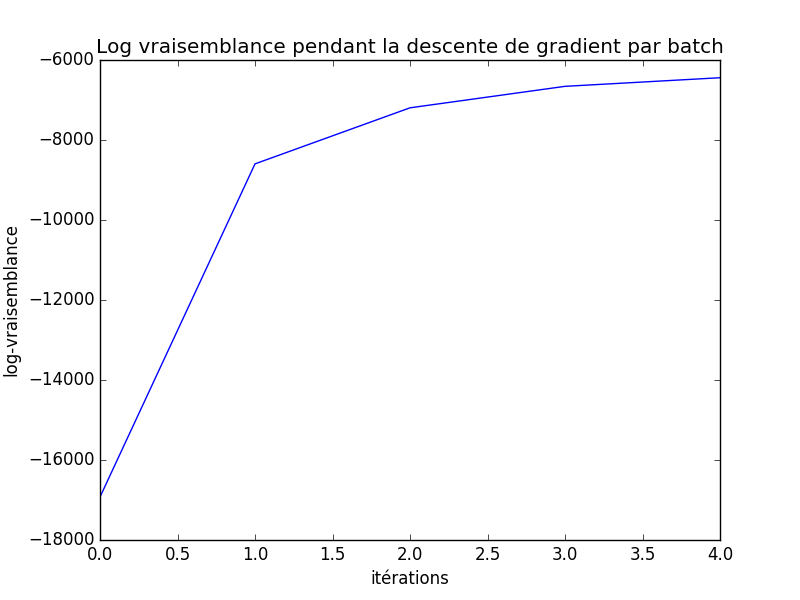
\includegraphics[scale=0.8]{img/mb_5_1_logv.png}
	\caption{Log-vraisemblance, taux = $\frac{5}{t+1}$}
\end{center}
\end{figure}


On voit donc que le taux d'apprentissage a le même impact que pour la version par "batch". Avec un taux plus grand, la descente de gradient se fait plus vite (3-4 itérations contre 10 itérations).

A nouveau, les valeurs finales pour la précision sont différentes mais il n'est pas possible de conclure sur quelque chose à ce niveau là. J'ai aussi utilisé un terme de régularisation afin de réduire la possibilité de sur-apprentissage, ainsi qu'un \textit{momentum} pour fluidifier l'optimisation. Le seuil utilisé pour la détection d'une convergence reste le même, c'est à dire 0.001. 
\\ \linebreak
Enfin, pour comparer les deux versions de la descente de gradient, j'affiche un graphe présentant la précision sur les trois ensembles dans les 2 cas. J'ai repris des taux d'apprentissage moyen : taux = 0.0005 et taux = $\frac{1}{t+1}$

\begin{figure}[H]
\begin{center}
	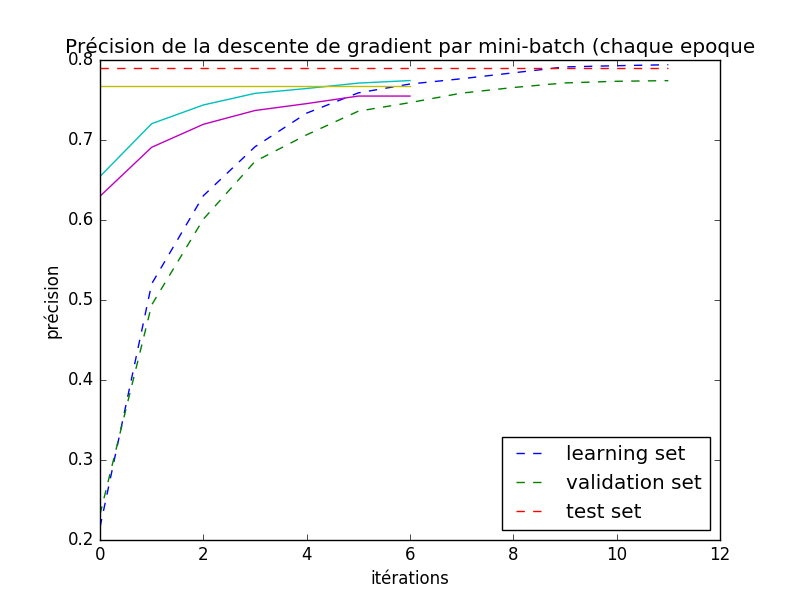
\includegraphics[scale=0.8]{img/comp_precision.png}
	\caption{Comparaison précision batch/mini-batch, $taux_{batch} = 0.0005$, $taux_{mini-batch} = \frac{1}{t+1}$}
\end{center}
\end{figure}
On voit donc bien que la version par mini-batch est plus rapide : 4-6 itérations contre 8-10.
Au niveau de la précision finale atteinte, on ne peut rien conclure. J'ai refait plusieurs fois les mesures et parfois la version par "batch" est meilleure et parfois c'est celle par "mini-batch". Dans tous les cas, la différence de précision entre les deux méthode est vraiment minime. 


On peut donc conclure que les "mini-batch" améliorent la performance de la régression logistique du point de vue de la vitesse. Le processus d'optimisation prend moins de temps, mais ne procure pas une meilleure précision. Avec un nombre de données plus important, la différence de rapidité serait d'après moi encore plus flagrante.
\end{document} 
